\chapter{Entorno virtual}
Uno de los principales objetivos del proyecto es realizar pruebas funcionales y de escala sobre la arquitectura del prototipo. Es de interés generar realidades distintas, y así detectar puntos de falla o variables clave en la performance de la arquitectura. Para esto se puede utilizar dos parámetros: topología y servicios. Es importante poder aplicar topologías complejas y relativamente grandes a la arquitectura, así como grandes cantidades de servicios para determinar qué niveles de tráfico o flujos soporta el sistema antes de fallar o ver su performance reducida drásticamente. Dado que no es realista hacer este tipo de pruebas con un prototipo físico, por temas económicos y prácticos, se observa la necesidad de un entorno virtual capaz de simular las características del prototipo.

\section{Requerimientos del entorno virtual}
En primer lugar, el objetivo es que el entorno virtual se comporte de una forma lo más cercana posible al prototipo físico. Esto no quiere decir que deba usar las mismas herramientas, pero es deseable que así sea. A estos requerimientos, se agregan los requisitos inherentes de un entorno de virtualización como el que se pretende. A continuación se detallan los principales requerimientos a tener en cuenta.
\begin{itemize} 
	\item OSPF. El prototipo es dependiente en que los routers puedan utilizar este protocolo de enrutamiento, entonces resulta crucial que los nodos virtuales también puedan.
	\item OpenFlow 1.3: La aplicación que implementa VPNs sobre el prototipo depende de que los switches OpenFlow tengan soporte para MPLS, y OpenFlow ofrece MPLS a partir de la versión 1.3 (???).
	\item Facilidad de configurar: Es importante que el entorno pueda generar distintas topologias y escenarios sin demasiado esfuerzo de configuración.
	\item Escalabilidad: Dado que uno de los objetivos es realizar pruebas de escala, el entorno debería ofrecer buena escalabilidad. Esto se traduce a que una computadora promedio de uso personal pueda levantar una decena de nodos virtuales como mínimo.
\end{itemize}

\section{Herramientas candidatas}
Se estudió el estado del arte en lo que respecta a opciones de emulación o simulación para SDN. A continuación se detallan las principales herramientas analizadas al momento de hacer esta investigación.\\

\textbf{NS-3}\\
ns-3 fue descartado debido a que no ofrece soporte para Quagga ni OpenFlow 1.3 al momento de realizar esta investigacion.\\

\textbf{Estinet}\\
Estinet requiere licencias pagas, y se opto por elegir herramientas open source. Debido a la falta de documentación de libre acceso, no se sabe que tipo de capacidades ofrece.\\

\textbf{Mininet}\\
Mininet es un emulador de redes SDN que permite emular hosts, switches, controladores y enlaces. Utiliza virtualización basada en procesos para ejecutar múltiples instancias (hasta 4096) de hosts y switches en un unico kernel de sistema operativo. También utiliza una capacidad de Linux denominada \textit{network namespace} que permite crear "interfaces de red virtuales", y de esta manera dotar a los nodos con sus propias interfaces, tablas de ruteo y tablas ARP. Lo que en realidad hace Mininet es utilizar la arquitectura \textit{Linux container}, que tiene la capacidad de proveer virtualización completa, pero de un modo reducido ya que no requiere de todas sus capacidades. Mininet también utiliza \textit{virtual ethernet (veth)} para crear los enlaces virtuales entre los nodos.


\textbf{LXC}\\
La opción de crear nodos con Linux containers resuelve el problema de Quagga y OpenFlow 1.3, pero llevaría una gran cantidad de trabajo construir distintas topologias (sobre todo si son grandes), ya que casi todo debe ser configurado manualmente por el usuario. Es una opción similar a Mininet, solo que sin gozar de todas las facilidades que ofrece esta última.\\


\textbf{Máquinas virtuales}\\
Es una opción similar a LXC (Linux Containers), sólo que menos escalable.
\\

\section{Diseño e implementación del entorno}
El entorno está construido alrededor de Mininet, y se podría pensar como una extensión de la misma. \textit{Out of the box}, Mininet ya cumple tres de los cuatro requerimientos explicados anteriormente. Está diseñada para ser escalable, ya que usa containers reducidos, tiene soporte para OpenFlow 1.3 mediante OpenVSwitch, y es muy fácil de usar. El aspecto en el que falla es en el soporte para Quagga. Dado que Mininet es una herramienta de prototipado para SDN puro, no está pensado para un esquema híbrido como el que se propone. Los switches compatibles con OpenVSwitch que ofrece no pueden tener su propio network namespace, por lo tanto, no pueden tener su propia tabla de ruteo ni interfaces de red aisladas, así que no es posible que utilicen Quagga.

Por otro lado, los hosts de Mininet sí tienen su propio network namespace, y gracias a su capacidad de tener sus propios procesos y directorios, podemos ejecutar una instancia de Quagga y OpenVSwitch para cada host. De esta forma es posible crear un router como el requerido por la arquitectura. Esta extensión de las funcionalidades de los hosts es posible ya que Mininet está programado con orientación a objetos y permite al usuario crear subclases propias de las clases que vienen por defecto. En la figura \ref{fig:clases_entorno} se puede ver la estructura de clases del entorno construido. En las siguientes secciones se procederá a estudiar cada una de ellas.

\begin{figure}[t]
	\caption{Diagrama de clases del entorno.}
	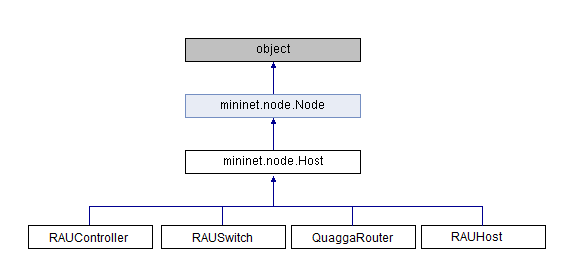
\includegraphics[scale=0.65]{Entorno/clases_entorno}
	\centering
	\label{fig:clases_entorno}
\end{figure}

\subsection{RAUController}
En el uso típico de Mininet, la comunicación entre el controlador y el switch se da a través de la interfaz de loopback. Esto es así porque los switches no tienen su propio namespace. Para lograr dicha comunicación, no hace falta un objeto en Mininet que represente el controlador, ya que ejecutar la aplicación en el sistema operativo base ya habilita al switch a comunicarse con ella a través de la interfaz de loopback. Esta situación cambia en este diseño, porque los switches pasan a tener su propio network namespace. Esto lleva a la necesidad de crear un host virtual, que ejecute la aplicación de RAUFlow y se comunique con los switches a través de enlaces virtuales. Para satisfacer esta necesidad se usa la clase RAUController.

\subsection{RAUSwitch}
La clase RAUSwitch es el núcleo del entorno de simulación. Es un Host extendido de tal forma para que, gracias a la funcionalidad de directorios privados, ejecute su propia instancia de Quagga y OpenVSwitch. Cada RAUSwitch tiene los siguientes directorios privados: /var/log/, /var/log/quagga, /var/run, /var/run/quagga, /var/run/openvswitch. Cada RAUSwitch también usa un directorio bajo /tmp, para almacenar sus archivos de configuración.\\ \\

OpenVSwitch básicamente consiste de 2 demonios (ovs-vswitchd y ovsdb-server) que ejecutan en el user-space, y un módulo en el kernel que actúa como cache para los flujos recientes. Utiliza el protocolo 'netlink' para comunicar el user-space con el módulo en el kernel. Poder tomar decisiones sobre los paquetes a nivel del kernel, sin tener que pasar por el user-space, explica en gran medida el buen nivel de performance que ofrece OpenVSwitch. Sin embargo, tener múltiples módulos de kernel ejecutando en el mismo sistema operativo puede crear comportamientos impredecibles e incorrectos, ya que no está previsto para trabajar de esa forma.\\
Afortunadamente, OpenVSwitch puede ejecutarse completamente en modo user-space, es decir, sin soporte del módulo del kernel. Esto implica que podemos ejecutar tantas instancias de OpenVSwitch como queramos, pero la performance va a ser significativamente peor. Esto no es una desventaja muy seria, ya que el objetivo del entorno no es ser performante al procesar paquetes. Cabe aclarar que en este modo OpenVSwitch continúa haciendo cacheo de flujos, pero ahora lo hace en el user-space.

\begin{figure}[t]
	\caption{Arquitectura de OpenVSwitch.}
	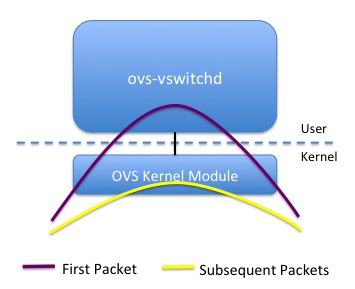
\includegraphics[scale=0.65]{Entorno/ovs_dataplane}
	\centering
	\label{fig:ovs_dataplane}
\end{figure}

\subsection{QuaggaRouter}
Es una clase similar al RAUSwitch pero sin OpenVSwitch, es decir, sólo usa Quagga. Apunta a representar el router CE que utilizaría una subred para conectarse a la red. Está conectado a un RAUSwitch de borde.

\subsection{RAUHost}
Es una clase auxiliar, sin ninguna particularidad. Sirve para evitar determinadas configuraciones manuales, como por ejemplo, el \textit{default gateway}.

